El sistema diseñado permite medir la masa de recipientes de hasta
\SI{1.5}{\kg} mediante una célula de carga resistiva de aluminio de
\SI{5}{\kg} de capacidad nominal \cite{loadcell_datasheet}.
La señal diferencial generada por el puente de Wheatstone se
acondiciona, digitaliza y procesa para obtener una lectura estable
en gramos.

% (excitación -> sensor -> filtro RFI -> AD623 -> DAQ -> LabVIEW)
\begin{figure}[H]
    \centering
    %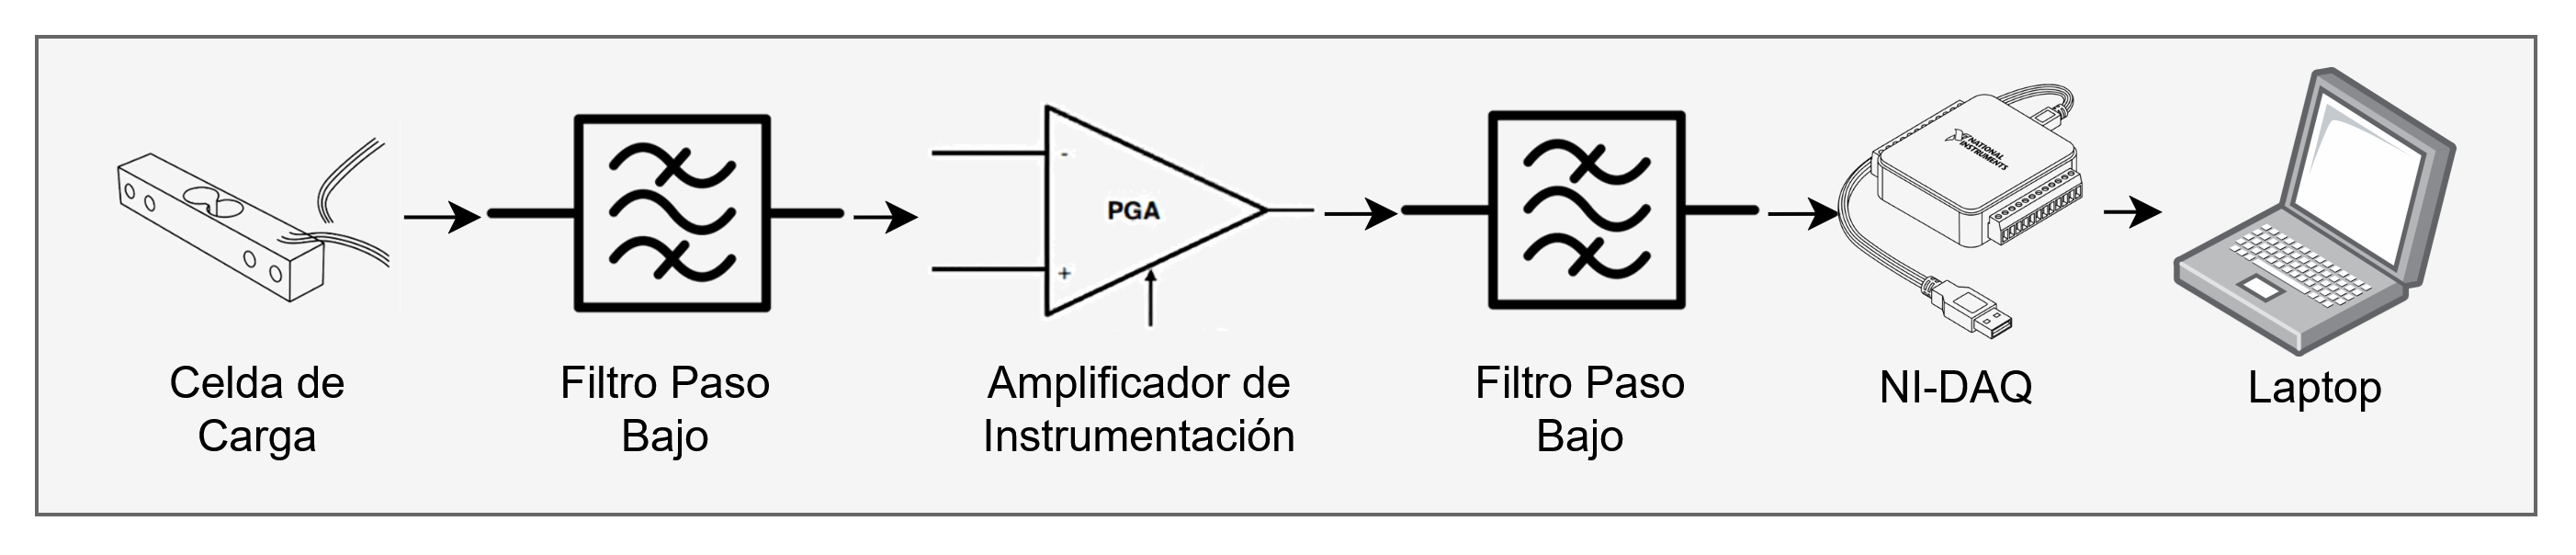
\includegraphics[width=0.85\textwidth]{figs/diagrama_bloques.png}
    \caption{Arquitectura general del sistema de pesaje a nivel de bloques.}
    \label{fig:bloques}
\end{figure}

\subsection{Objetivos}

El objetivo principal consiste en diseñar, montar y verificar una
báscula de precisión orientada al pesaje estático. De forma más
específica, se persigue:

\begin{itemize}
    \item Dimensionar analíticamente cada etapa del acondicionamiento
          de señal.
    \item Garantizar márgenes de seguridad frente a la saturación
          del amplificador.
    \item Validar el modelo matemático con medidas reales en la
          \textit{protoboard}.
\end{itemize}

\subsection{Requisitos técnicos}

\begin{itemize}
    \item Rango de pesaje: de \SI{0}{\g} a \SI{1500}{\g}.
    \item Tensión de excitación estable de \SI{4.096}{\V}
          (MCP1541) \cite{microchip_mcp1525_2012}.
    \item Pedestal de referencia de \SI{1.0}{\V} para evitar
          saturación por desequilibrio negativo (MCP6021) \cite{mcp6021_datasheet}.
    \item Frecuencia de corte del filtro diferencial RFI próxima
          a \SI{5}{\Hz}.
    \item Adquisición en modo diferencial en la NI USB-6001
          \cite{ni6001_datasheet}.
\end{itemize}